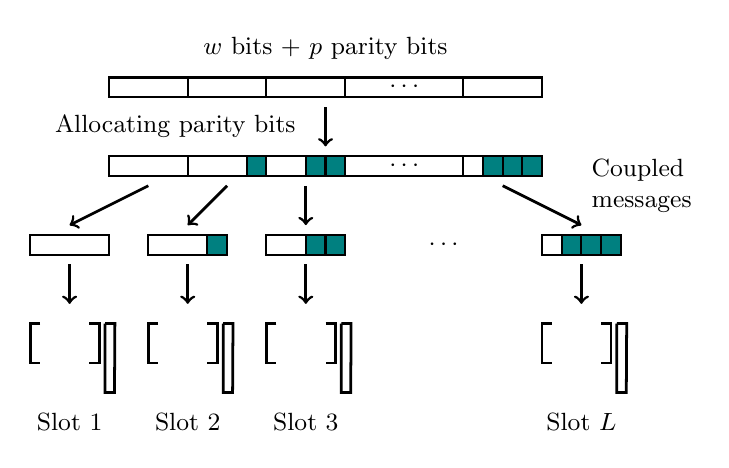
\begin{tikzpicture}
[font=\small, draw=black, line width=0.75pt,
sub0/.style={rectangle, draw, inner sep=0pt, minimum width=10mm,  minimum height=2.5mm},
sub1/.style={rectangle, draw, inner sep=0pt, minimum width=15mm, minimum height=2.5mm},
sub1s/.style={rectangle, inner sep=0pt, minimum width=15mm, minimum height=2.5mm},
parity/.style={rectangle, draw, fill=teal, inner sep=0pt, minimum size=2.5mm}]

\node (coupledvector) at (2.25,5.50) {$w$~bits + $p$~parity bits};
\node[sub0] (cs0) at (0.00,5) {};
\node[sub0] (cs2) at (1.00,5) {};
\node[sub0] (cs3) at (2.00,5) {};
\node[sub1] (csx) at (3.25,5) {$\cdots$};
\node[sub0] (csz) at (4.50,5) {};

\draw[->, line width=1pt]  (2.25,4.75) -- (2.25,4.25);
\node[anchor=east] (coding) at (2.00,4.50) {Allocating parity bits};

\node[sub0] (subcs0) at (0.00,4) {};
\node[sub0] (subcs2) at (1.00,4) {};
\node[parity] (parity0) at (1.375,4) {};
\node[sub0] (subcs3) at (2.00,4) {};
\node[parity] (parity1) at (2.125,4) {};
\node[parity] (parity2) at (2.375,4) {};
\node[sub1] (subcsx) at (3.25,4) {$\cdots$};
\node[sub0] (subcsz) at (4.50,4) {};
\node[parity] (parity3) at (4.375,4) {};
\node[parity] (parity4) at (4.625,4) {};
\node[parity] (parity5) at (4.875,4) {};

\node[sub0] (subcs0) at (-1.00,3) {};
\node[sub0] (subcs2) at (0.50,3) {};
\node[parity] (parity0) at (0.875,3) {};
\node[sub0] (subcs3) at (2.00,3) {};
\node[parity] (parity1) at (2.125,3) {};
\node[parity] (parity2) at (2.375,3) {};
\node[sub1s] (subcsx) at (3.75,3) {$\cdots$};
\node[sub0] (subcsz) at (5.50,3) {};
\node[parity] (parity3) at (5.375,3) {};
\node[parity] (parity4) at (5.625,3) {};
\node[parity] (parity5) at (5.875,3) {};

\draw[->, line width=1pt]  (0.00,3.75) -- (-1.00,3.25);
\draw[->, line width=1pt]  (1.00,3.75) -- (0.50,3.25);
\draw[->, line width=1pt]  (2.00,3.75) -- (2.00,3.25);
\draw[->, line width=1pt]  (4.50,3.75) -- (5.50,3.25);
\node[anchor=west,align=left] (coupledvector) at (5.50,3.75) {Coupled\\messages};

\foreach \v in {-1.00,0.50,2.00,5.50} {
  \draw[->, line width=1pt]  (\v,2.75) -- (\v,2.25);

  \draw[line width=1pt] (\v-0.375,2) -- (\v-0.5,2) -- (\v-0.5,1.5) -- (\v-0.375,1.5);
  \draw[line width=1pt] (\v+0.25,2) -- (\v+0.375,2) -- (\v+0.375,1.5) -- (\v+0.25,1.5);
  \draw[line width=1pt] (\v+0.45,2) -- (\v+0.45,1.125) -- (\v+0.57,1.125) -- (\v+0.575,2) -- (\v+0.45,2);
}

\node (cs) at (-1.00,0.75) {Slot~1};
\node (cs) at (0.50,0.75) {Slot~2};
\node (cs) at (2.00,0.75) {Slot~3};
\node (cs) at (5.50,0.75) {Slot~$L$};
\end{tikzpicture}
